\section{Python AIMA}

\begin{enumerate}
    \item In order to perform a search, what are the classes that you
        must define or extend? Explain precisely why and where they are
        used inside a tree\_search.
        \begin{framed}
            The only class we need to extend is the class Problem because
            it is an abstract class and it doesn't exactly fit our purpose.
            This class is used by all the uninformed searchs. In
            tree\_search (called by breadth\_first\_tree\_search and
            depth\_first\_tree\_search), the first argument is a Problem,
            which is an object from the class Problem. It is needed to get
            an initial state from the problem to create the first node, do a search (this one
            depends on the data structure used for the fringe), testing
            for every node if the current node is the goal we have to
            reach and every loop expands the tree with the node directly
            linked from the visited node (thanks to the Problem.successor
            method).
        \end{framed}
    \item In the expand method of the class Node what is the advantage
        of using a yield instead of building a list and returning it
        afterwards ?
        \begin{framed}
            The advantage is that \textit{yield} builds a list item-by-item, it is
            some kind of lazy programming that permits to create only the
            nodes that are really used by our program, it is very useful to
            avoid a too large memory usage than what is needed.
        \end{framed}
    \item Both breadth\_first\_graph\_search and depth\_first\_graph\_search
        are making a call to the same function. How is their fundamental
        difference implemented?
        \begin{figure}[!ht]
        \begin{framed}
            The fundamental difference is that the data structure used is
            totally different :
            \begin{description}
                \item[Breadth-first graph search] needs a FIFOQueue as a
                    data structure because while the graph\_search is
                    performed, it expands the nodes linked to the visited
                    nodes, a FIFO (first in, first out) queue allows the
                    path to follow the root node then the nodes linked to
                    the root node, then the nodes linked to the previous
                    node, as shown on the next figure.
                \item[Depth-first graph search] needs a LIFO (last in,
                    first out) queue, in other words a Stack, because it
                    must always first follow the last expansion of the
                    nodes visited before until the goal is reached or the
                    branch of the tree cannot lead to a goal state. The
                    comportement of this function is shown on the next
                    figure.
            \end{description}
                \centering
                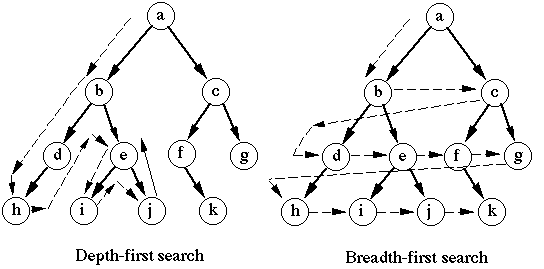
\includegraphics[width=0.75\linewidth]{depth_or_breadth.png}
                \caption{Difference between a breadth-first and a depth-first
                search algorithm, here represented for a tree, but for a
                graph it works the same (but you can have symmetric state,
                cycles)}
        \end{framed}
        \end{figure}
        \FloatBarrier
    \item What is the difference between the implementation of the
        graph\_search and the tree\_search methods and how does it impact
        the search methods ?
        \begin{framed}
            The only difference is that graph\_search method maintains a
            closed list (a dictionary) that keeps in memory all the states
            already visited, because graphs can contains symmetric states
            and we need to avoid the search to loop in cycles in the graph
            (because it doesn't provide any useful additional information).
        \end{framed}
    \item What kind of structure is used to implement the closed list?
        What are the methods involved in the search of an element inside
        it? What properties must thus have the elements that you can put
        inside the closed list ?
        \begin{framed}
            It's a dictionary, it takes an hashable object as index and
            every index is linked to a variable. The \verb#if node.state not in closed#
            instruction checks whether \verb#node.state# is already an
            index of the closed list (then this instruction would be
            false) or not (then this instruction would be true).
        \end{framed}
    \item How technically can you use the implementation of the closed
        list to deal with symmetrical states ? (hint: if two symmetrical
        states are considered by the algorithm to be the same, they will
        not be visited twice)
        \begin{framed}
            The hash function for the \verb#node.state# must always return
            a unique result that permits a comparison between two object
            and thats returns True when two states are symmetric.
        \end{framed}
\end{enumerate}

\section{The Numberlink Problem}

\begin{enumerate}
    \item Explain the advantages and weaknesses of the following search
        strategies on this problem (not in general): depth first,
        breadth first.
        \begin{framed}
            The breadth-first search expands the shallowest unexpanded node
            and implements the frontier as a FIFO Queue. In this problem,
            it means that we will check every path possible for one letter,
            then check every path possible for a second letter, and so on
            (without following the branches that couldn't reach to the
            goal). The main advantage is that we can work one letter at a
            time and be sure that all the paths for a letter have already
            been visited once at the moment we try another letter, the main
            disadvantage is the space this search needs (because we have to
            keep the paths followed from the root to each node) and if the
            directions given give a good heuristic, we will not take
            advantage of it. \newline

            The depth-first search expands the deepest unexpanded node and
            implements the frontier as a LIFO Queue. In this problem, it
            means that we try to reach as soon as possible a viable path
            for the first letter, then for the second, and so on (withtout
            following the branches that couldn't reach to the goal). The
            main advantages are that : first, if we have a good heuristic, the path to
            the goal will be found quickly; second, the memory space isn't
            a problem here because even if we have to keep the full path
            from root node to the node, it is only the current path that is
            kept in memory. The main disadvantage is that our successor
            method must be very well implemented to highlight the sooner as
            it can a branch that can't anymore reach a goal state, because
            that kind of search can lead us to a node far from the goal
            node (a poorly implemented algorithm can lead to a very long
            time to discover the solution)
        \end{framed}
    \item How can we exploit the uniqueness of solution to reduce the
        search space? Why is the method pathExists useful ?
        \begin{framed}
            We can exploit the uniqueness of solution to avoid states that
            wouldn't be a solution in a well-designed problem (for example,
            a 2x2 grid in our state with the same letter will never
            lead to a goal for a well-designed problem). Likewise, a state
            that doesn't permit all the other letters to be connected by
            their two endpoints are not leading to a goal state (and that's
            why the method pathExists is made for).
        \end{framed}
    \item Is the order in which we choose the paths important? How can
        we use this to reduce the search space? When starting a new
        path, we can choose to start with any of its two endpoint. How
        should this choice be done ?
        \begin{framed}
            As it is an uninformed search, we can never be sure that the
            order is important. But if it is imposed to us, we assume that
            it will help us to reduce the search space by giving us a good
            heuristic method. We thought about some improvements, like starting by the letter with
            the shortest length between its endpoints but it doesn't provide any better result than the
            basic technique so we don't think that really matters for this
            assignment.
        \end{framed}
    \item What are the advantages and disadvantages of using the tree
        and graph search for this problem. Which approach would you
        choose? Which approach allows you to avoid expending twice
        symmetrical states ?
        \begin{framed}
            The advantage of the graph search over the tree search is that
            this first one avoid expending twice symmetrical states. The
            disadvantage of this method is that (in this implementation)
            the state must be hashable (to be an index in the closed list)
            while it must be a grid that is not hashable (to be used in the pathExists
            method) so we would have to maintain two data structures
            containing the exact same information if we use the graph
            search. As we couldn't think of any symmetrical state when we
            use the fact that we won't extend a state that would contain a
            2x2 grid containing the same letter 4 times and that we will
            always start by the same endpoint, the tree search would be a
            better approach.
        \end{framed}
    \item Implement this problem in Python 3. Extend the Problem class
        and implement the necessary methods and other class(es) if
        necessary. Your file must be named numberlink.py. You program
        must take as only input the path to the init file of the problem
        to solve. It must print to the standard output a solution to the
        problem satisfying the above format. Your file must be encoded
        in utf-8. Submit your program on INGInious.
        \begin{figure}[!ht]
            \begin{framed}
                \centering
                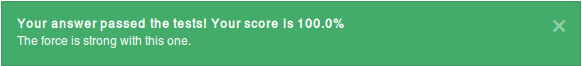
\includegraphics[width=0.85\linewidth]{inginious.png}
            \end{framed}
        \end{figure}
        \FloatBarrier
    \item Experiments must be realized with the 10 instances of the
        numberlink problem provided. Report in a table the results on
        the 10 instances for depth-first and breadth- first strategies
        on both tree and graph search (4 settings). You must report the
        time, the number of explored nodes and the number of steps from
        root to solution. When no solution can be found by a strategy in
        a reasonable time (3 min), explain the reason (time-out and/or
        swap of the memory). What do you conclude from those experiments
        ?
	\begin{framed}
	  \begin{tabular}{l|l|l|l|l}
	    & Depth, tree & Depth, graph & Breadth, tree & Breadth, graph \\
	    \hline
	    easy & 30ms & 30ms &  & 30ms \\
	    level2m & 2m56 & 18s31 & & 1m19 \\
	    level4m & 80ms & 660ms & & 360ms \\
	    level9m & 210ms & 320ms & & 610ms \\
	    level10m & 4m21 & 3m25 & & 8m06\\
	    level15m & 3m07 & 3m52 & & \\
	    level38s & 120ms & 240ms & & \\
	    level39s & 1s15& 80ms & & \\
	    path & 70ms & 120ms & & \\
	    wiki & 50ms & 90ms & & \\
	  \end{tabular}
	\end{framed}

\end{enumerate}
